\documentclass{amsart}
\usepackage{mmap} % make PDF files generated by pdfLaTeX both searchable and copy-able in acrobat reader and other compliant PDF viewers
\usepackage{amssymb}
\usepackage{graphicx}
\usepackage{hyperref}
\usepackage{enumerate}

\usepackage{etextools}[2010/12/07]
%===== restore etoolbox definition of \forlistloop =====
\makeatletter
\renewcommand*{\forlistloop}[2]{%
  \expandafter\etb@forlistloop\expandafter{#2}{#1}}
%====================== end fixes ======================

\usepackage{aliascnt}

\usepackage{amssymb}
%================================ AMSTHM ================================
\swapnumbers

% makes \autoref work right
% env_name numbered_like caption
\def\newaliasedtheorem#1[#2]#3{
  \newaliascnt{#1}{#2}
  \newtheorem{#1}[#1]{#3}
  \aliascntresetthe{#1}
  \expandafter\providecommand\expandafter*\expandafter{\csname #1autorefname\endcsname}{#3}
}

\newtheorem{thm}{Theorem}[section]
%\newtheorem{theorem}{Theorem}
\newaliasedtheorem{conjecture}[thm]{Conjecture}
\newaliasedtheorem{lem}[thm]{Lemma}
%\newtheorem{lemma}[theorem]{Lemma}
\newaliasedtheorem{cor}[thm]{Corollary}
%\newtheorem{corollary}[theorem]{Corollary}
\newaliasedtheorem{prop}[thm]{Proposition}
%\newtheorem{proposition}[theorem]{Proposition}
%\newtheorem{definition}[theorem]{Definition}
%\newtheorem{example}[theorem]{Example}
%\newtheorem{exercise}[thm]{Exercise}
%\newtheorem{exercise}[theorem]{Exercise}
\newaliasedtheorem{claim}[thm]{Claim}
\newaliasedtheorem{law}[thm]{Law}
\newtheorem*{thm*}{Theorem}
\newtheorem*{lem*}{Lemma}
\newtheorem*{conjecture*}{Conjecture}
\newtheorem*{cor*}{Corollary}
\newtheorem*{prop*}{Proposition}
\newtheorem*{exercise*}{Exercise}
\newtheorem*{law*}{Law}
\newtheorem*{claim*}{Claim}


\theoremstyle{definition} \newaliasedtheorem{defn}[thm]{Definition}
\theoremstyle{definition} \newtheorem*{defn*}{Definition}
\theoremstyle{definition} \newaliasedtheorem{xca}[thm]{Exercise}
\theoremstyle{definition} \newtheorem*{soln*}{Solution}
\theoremstyle{definition} \newaliasedtheorem{remark}[thm]{Remark}
\theoremstyle{definition} \newtheorem*{remark*}{Remark}
\newaliasedtheorem{example}[thm]{Example}
\newtheorem*{example*}{Example*}
\newaliasedtheorem{examples}[thm]{Examples}
\newtheorem*{examples*}{Examples}
\newaliasedtheorem{eg}[thm]{Example}
\newtheorem*{eg*}{Example}

\newaliasedtheorem{fact}[thm]{Fact}
\newtheorem*{fact*}{Fact}
%============================== End AMSTHM ==============================

\newcommand{\defnlabel}[2][]{%
  \ifempty{#1}{%
    \label{defn:#2}\emph{#2}%
  }{%
    \label{defn:#1}\emph{#2}%
  }%
}

\newcommand{\defnref}[2][]{%
  \ifempty{#1}{%
    \hyperref[defn:#2]{#2}%
  }{%
    \hyperref[defn:#1]{#2}%
  }%
}

\usepackage[all]{xy}

\let\from=\leftarrow

\newcommand{\cat}[1]{\ensuremath{\mathbf{#1}}}
\DeclareMathOperator{\Ob}{Ob}
\DeclareMathOperator{\Mor}{Mor}
\DeclareMathOperator{\id}{id}
\DeclareMathOperator{\Hom}{Hom}
\DeclareMathOperator{\colim}{colim}

\begin{document}
\title{A gentle introduction to a model category of topological spaces}
\author[J. Gross]{Jason Gross}
\address{Massachusetts Institute of Technology}
\email{\href{mailto:jgross@mit.edu}{jgross@mit.edu}}
\date{\TeX ed on \today}
%\subjclass[2000]{Primary 18B30; Secondary 54-01}
%Primary: Categories of topological spaces and continuous mappings
%Secondary: General topology -- Instructional exposition (textbooks, tutorial papers, etc.)
%\thanks{}
%\keywords{Quillen,model category,topology,model structure}

\begin{abstract}
  The intent of this paper is to provide a gentle introduction to a model category of topological spaces.  The presentation is intended to be accessible to anyone familiar with introductory topology, homotopy, and CW-complexes.  In particular, no knowledge of category theory is assumed.  This paper introduces and explains all of the neccesary category theory to understand model categories; defines a model category; presents a model category structure for the category of topological spaces using homotopy equivalences, closed Hurewicz fibrations, and Hurewicz cofibrations; and elaborates on the axioms in the context of this particular model category.
\end{abstract}

\maketitle

\section{Introduction}
  The language of category theory is a powerful tool for describing properties and constructions that are the same in many fields of math.  The ``model category'' structures developed by Quillen provide a way to do much of homotopy theory in the more general setting of categories.  This paper aims to provide a gentle introduction to the theory of model categories, focusing on topological spaces as the primary example.
  
  We begin with an overview of the category theory necessary to fully understand the language used in specifying the axioms of a model category.  No prior exposure to category theory is assumed.  After that, we briefly review the topology necessary for describing the category of topological spaces as a model category.  I then state the axioms of a model category, and elaborate on them.
  
  This paper is largely based on Dwyer and Spalinski's \emph{Homotopy theories and model categories} (\cite{dwyer1995homotopy}), and is structured similarly.  Dwyer and Spalinski provide a much more in-depth introduction to the theory of model categories, though it is much more terse and assumes familiarity with the language of category theory.  I have included excercises throughout the section on category theory, either constructed for this paper, or taken from \cite{commutative_algebra} and \cite{sets_maps_limits_colimits}.  They are intended to help the reader grasp the material better.  They are intentionally not difficult, nor are they necessary to the development of the material.  Solutions are provided at the end of this paper; the reader is strongly encouraged to try the exercises before looking at the solutions.

\section{Category Theory}
  \begin{defn}[Category]
    A \defnlabel{category} $\cat C$ is a collection of \emph{objects}, denoted $\Ob(\cat C)$, together with a collection of \emph{morphisms} between objects (also called \emph{maps} or \emph{arrows}), subject to the following axioms:
    \begin{itemize}
      \item Morphisms may be composed:  If $f: X \to Y$ and $g : Y \to Z$ are morphisms in \cat C, then there is a morphism $g \circ f : X \to Z$.  We drop the $\circ$ when there is no ambiguity, and write $gf$ instead of $g \circ f$.
      \item Composition of morphisms is associative:  If $f: X \to Y$, $g: Y\to Z$, and $h: Z\to W$ are morphisms in \cat C, then $h \circ (g \circ f) = (h \circ g) \circ f$.
      \item Every object has an identity morphism:  For every object $X$, there is a morphism $\id_X : X \to X$ such that for every object $Y$, for every morphism $f : X \to Y$ and every morphism $g : Y \to X$, $f \circ \id_X = f$ and $\id_X \circ g = g$.
    \end{itemize}
    
    For any two objects $X$ and $Y$ in $\cat C$, we denote the collection of all morphisms $f: X \to Y$ in $\cat C$ by $\Hom_{\cat C}(X, Y)$.  In this paper, $\Hom_{\cat C}(X, Y)$ will always be a set (rather than something larger, like a collection or a class).
  \end{defn}
  
  \begin{remark*}
    The identity morphisms in any category are unique.  A morphism $f : X \to Y$ is called an \defnlabel{isomorphism} if there is a morphism $g : Y \to X$ such that $gf = \id_X$ and $fg = \id_Y$.  In this case, we say that $X$ and $Y$ are \defnlabel{isomorphic}.
  \end{remark*}
  
  \begin{examples*}\par\noindent
    \begin{itemize}
      \item The empty category, $\emptyset$, consisting of no objects and no morphisms
      \item The category, $*$, with one object and no non-identity morphisms.
      \item A category with a set $S$ of objects and no non-identity morphisms
      \item The category $\{a \from b \to c\}$ consisting of three objects, the two morphisms $b \to a$ and $b \to c$, and the three identity morphisms $\id_a$, $\id_b$, and $\id_c$
      \item The category \cat{Set}, consisting of sets (the objects) and maps between sets (the morphisms)
      \item The category \cat{Top}, consisting of topological spaces (the objects) and continuous maps (the morphisms)
      \item The category \cat{Grp}, consisting of groups (the objects) and maps preserving the group operation (the morphisms)
      \item For any two categories $\cat C$ and $\cat D$, there is a direct product category $\cat C \times \cat D$.  The objects are pairs of objects $(X, Y)$ for $X\in \Ob (\cat C)$ and $Y\in \Ob(\cat D)$ and the morphisms are pairs of morphisms $(f, g)$ for $f$ a morphism in $\cat C$ and $g$ a morphism in $\cat D$.
    \end{itemize}
  \end{examples*}
  
  \begin{defn}[Subcategory]
    If $\cat C$ and $\cat D$ are categories with $\Ob(\cat D) \subset \Ob(\cat C)$ and for which every morphism in $\cat D$ is also a morphism in $\cat D$, then we say that $\cat D$ is a \defnlabel{subcategory} of $\cat C$ and we write $\cat D \subset \cat C$.
  \end{defn}
  
  \begin{defn}[Initial and Terminal Objects]
    An \defnlabel{initial object} $\emptyset$ of a category $\cat C$ is an object with exactly one morphism \emph{to} every other object in $\cat C$.
    
    A \defnlabel{terminal object} $*$ of a category $\cat C$ is an object with exactly one morphism \emph{from} every other object $\cat C$.
  \end{defn}
  
  \begin{xca} \label{xca:initial_terminal_unique}
    Show that the initial and terminal objects of a category, if they exist, are unique up to unique \defnref{isomorphism}.
    
    (Solution on \autopageref{sol:initial_terminal_unique}.)
  \end{xca}
  
  \begin{examples*}\par\noindent
    \begin{itemize}
      \item The initial object in the category \cat{Set} of sets is the empty set; there is exactly one map from the empty set to any other set (the trivial one).  Furthermore, the empty set is the only set with a map to the empty set, so there are no other initial objects.
      \item Any singleton set (a set with one element) is a terminal object in the category \cat{Set}.  There is only one singleton set, up to unique isomorphism.
      \item The initial object in the category \cat{Top} of topological spaces is the empty space.  Any one-point space is a terminal object.
      \item In the category \cat{Grp} of groups, the (trivial) group with one element is both an initial object and a terminal object.
      \item The initial object in the category of groups is the group with one element.
      \item In the category of pointed sets (sets with a distinguished element), a morphism from $(A, a) \to (B, b)$ (with $a\in A$ and $b\in B$) is a map $f : A \to B$ with $f(a) = b$.  In this category, singleton sets are both initial and terminal objects.
      \item In the category of rings, the ring of integers $\mathbb Z$ is an initial object, and the trivial ring consisting of a single element $0 = 1$ is a terminal object.
      \item In the category of \defnref[small category]{small categories}, where the objects are small categories and the morphisms are \defnref[functor]{functors} between categories, the empty category is an initial object and the category $*$, with one object and no non-identity morphisms, is a terminal object.
    \end{itemize}
    See \cite{wiki:InitialAndTerminalObjects} for a more extensive list.
  \end{examples*}
  
  For ease of presentation, I now define categorical diagrams.  I will come back to these later to give a more precise characterization.
  
  \begin{defn}[Commutative Diagram]
    A \defnlabel{diagram} is a set of objects together with morphisms between those objects, subject to the same axioms as a category.  Diagrams may be thought of a picking specific objects from a category, or may be thought of as (usually small) subcategories of a particular category.
    
    If it is the case that, for any objects $X$ and $Y$ in the diagram, there is at most one morphism $f : X \to Y$ (i.e., $f : X \to Y$ is unique, if it exists), then that diagram is said to \defnlabel[commutative diagram]{commute}.  Informally, a commutative diagram is one in which all the ways that you can follow arrows to get from $X$ to $Y$ agree on how elements of $X$ get mapped to elements of $Y$.
  \end{defn}
  
  \begin{examples*}\par\noindent
    \begin{itemize}
      \item Any diagram with no non-identity morphisms is commutative.
      \item The following diagram, where incl.~denotes inclusion, is commutative:
        \[
          \xymatrix{
            \{1, 2, 3\} \ar@{^(->}[rr]^{\text{incl.}} \ar[dr]^{\times 2} && \{0, 1, 2, 3, \ldots\} \\
            & \{0, 2, 4, 6, 8, \ldots\} \ar[ur]^{\times \frac12}
          }
        \]
      \item The following diagram is not commutative:
        \[
          \xymatrix{
            \{1, 2, 3\} \ar@{^(->}[rr]^{\text{incl.}} \ar[dr]^{\times 2} && \{0, 1, 2, 3, \ldots\} \\
            & \{0, 2, 4, 6, 8, \ldots\} \ar@{^(->}[ur]^{\text{incl.}}
          }
        \]
    \end{itemize}
  \end{examples*}
  
  \begin{defn}[Functor]
    A functor is a map between categories.  More formally, a \defnlabel[functor]{(covariant) functor} $F : \cat C \to \cat D$ between two categories $\cat C$ and $\cat D$ is a map $F_{\Ob} : \Ob(\cat C) \to \Ob(\cat D)$ together with a map $F_{\Mor} : \Mor(\cat C) \to \Mor(\cat D)$ that is compatible with morphism composition in \cat C and \cat D.  That is, for any composable morphisms $f$, $g$ in $\cat C$, $F(fg) = F(f) F(g)$.
  \end{defn}
    
  In \defnref{diagram} notation, saying that $F$ is a functor is saying that for any objects $X$ and $Y$ and any morphisms $f: X \to Y$ and $g: Y \to Z$, the following diagram commutes:
  \[
    \xymatrix{
      X \ar[r]^f \ar[d]^F & Y \ar[r]^g \ar[d]^F & Z \ar[d]^F \\
      F(X) \ar[r]^{F(f)} & F(Y) \ar[r]^{F(g)} & F(Z)
    }
  \]
  
  Note that this implies that functors preserve identity morphisms.
  
  \begin{xca}[(6.3) in \cite{commutative_algebra}] \label{xca:functor_commutative_diagram}
    Show that a functor $F$ being compatible with morphism composition is eqivalent to the following diagram being commutative for all objects $X$, $Y$, and $Z$, and all morphisms $f: X \to Y$:
    \[
      \xymatrix{
        \Hom_{\cat C}(Y, Z) \ar[r] \ar[d] & \Hom_{\cat D}(F(Y), F(Z)) \ar[d] \\
        \Hom_{\cat C}(X, Z) \ar[r] & \Hom_{\cat D}(F(X), F(Z))
      }
    \]
    
    (Solution on \autopageref{sol:functor_commutative_diagram}.)
  \end{xca}
  
  \begin{example}[Forgetful Functors]
    Many categories admit a forgetful functor, usually to the category of sets.  For example, the map that sends a topological space to its set of points is a forgetful functor from \cat{Top} to \cat{Set}.
  \end{example}
  
  \begin{example}
    For any category $\cat C$, the identity functor $\id_{\cat C}: \cat C \to \cat C$ sends every object to itself and every morphism to itself.
  \end{example}
  
  \begin{defn}[Opposite Category]
    For any category $\cat C$, there is an \defnlabel{opposite category} $\cat C^\text{op}$ which has the same objects as $\cat C$, but in which all the arrows are reversed.  That is, for any morphism $f : X \to Y$ in $\cat C$, there is an opposite morphism $f^\text{op} : Y \to X$ in $\cat C^\text{op}$.  Composition is given by the rule $f^\text{op}g^\text{op} = (gf)^\text{op}$.
  \end{defn}
  
  A functor $F: \cat C^\text{op} \to \cat D$ is also called a \defnlabel{contravariant functor} $\cat C \to \cat D$.
  
  \begin{xca} \label{xca:hom_op}
    The assignment of pairs of objects $(X, Y) \mapsto \Hom_{\cat C}(X, Y)$ gives a functor
    \[
      \Hom_{\cat C}(-, -) : \cat C^\text{op} \times \cat C \to \cat{Set}
    \]
    
    Why is this a functor from $\cat C^\text{op} \times \cat C$, rather than from $\cat C \times \cat C$, $\cat C \times \cat C^\text{op}$, or $\cat C^\text{op} \times \cat C^\text{op}$?
    
    (Solution on \autopageref{sol:hom_op}.)
  \end{xca}
  
  \begin{defn}[Natural Transformation]
    A \defnlabel{natrual transformation} is a map between functors that is compatible with how the functors act on morphisms.  More formally, given two functors $F, F' : \cat C \rightrightarrows \cat D$, a natrual transformation $t : F \to F'$ is a collection of maps $t_X : F(X) \to F'(X)$ (one for each object $X$ of $\cat C$) such that $t_YF(f) = F'(f)t_X$ for every map $f: X \to Y$ of $\cat C$.  This is equivalent to saying that the following diagram is commutative:
    \[
      \xymatrix{
        F(X) \ar[r]^{F(f)} \ar[d]^{t_X} & F(Y) \ar[d]^{t_Y} \\
        F'(X) \ar[r]^{F'(f)} & F'(Y)
      }
    \]
  \end{defn}
  
%  \begin{defn}[Natural Equivalence]
%    A \defnlabel{natrual equivalence} is a natrual transformation $t$ such that $t_X : F(X) \to F'(X)$ is an isomorphism in $\cat D$ for every object $X$ of $\cat C$.
%  \end{defn}
  
  \begin{defn}[Small and Finite Categories]
    A category $\cat D$ is called \defnlabel[small category]{small} if its collection of objects $\Ob(\cat D)$ is a set (rather than proper class or some larger collection).  A category $\cat D$ is called \defnlabel[finite category]{finite} if its collection of objects $\Ob(\cat D)$ is a finite set, and there are a finite number of morphisms between any two objects.
  \end{defn}
  
  \begin{defn}[Functor Categories and Diagrams]
    If $\cat C$ is a category and $\cat D$ is a small category, then the \defnlabel{functor category} $\cat C^{\cat D}$ consists of the collection of functors $F : \cat D \to \cat C$ (objects) and natrual transformations between these functors (morphisms).  This is also called the category of \emph{diagrams in \cat C with the shape of \cat D}.
  \end{defn}
  
  \begin{example}
    If $\cat D$ is the category $\{a, b\}$ (a category with two objects and no non-identity morphisms), then the objects in $\cat C^{\cat D}$ are commutative diagrams consisting of exactly two objects and no non-identity morphisms.
  \end{example}
  
  \begin{example}
    Recall that $\emptyset$ is the category with no objects.  The unique object in $\cat C^\emptyset$ is the empty commutative diagram consisting of no objects.
  \end{example}
  
  \begin{example}
    Recall that $*$ is the category with one object and no non-identity morphisms.  The objects in $\cat C^{*}$ are commutative diagrams consisting of one object and no non-identity morphisms.  We call such diagrams \defnlabel[constant diagram]{constant diagrams}.
  \end{example}
  
  \begin{example}
    If $\cat D$ is the category $\{a \to b\}$, then the objects in $\cat C^{\cat D}$ are commutative diagrams $X_a \to X_b$, and the morphisms are natrual transformations $t$ which make the following diagram commute:
    \[
      \xymatrix{
        X_a \ar[d]^f \ar[r]^{t_a} & Y_a \ar[d]^g \\
        X_b \ar[r]^{t_b} & Y_b
      }
    \]
    
    In this case, $\cat C^{\cat D}$ is called the \defnlabel{category of morphisms} of $\cat C$, which we denote by $\Mor(\cat C)$.
  \end{example}
  
  \begin{example}
    Suppose $\cat D$ and $\cat D'$ are small categories and $F : \cat D \to \cat D'$ is a functor.  Then $F$ gives a map $\cat C^{\cat D'} \to \cat C^{\cat D}$.  That is, for any $D' \in \cat C^{\cat D'}$, composition gives that $D'F \in \cat C^{\cat D}$ is a diagram with the shape of $\cat D$:
    \[
      \xymatrix{
        \cat D \ar@{.>}[dr]^{D} \ar[d]_F & \\
        \cat D' \ar[r]_{D'} & \cat C \\
      }
    \]
  \end{example}
  
  \begin{example} \label{ex:constant_diagram_category}
    Let $\cat D$ be a small category, and recall that $*$ is the category with one object and no non-identity morphisms.  Since $*$ is the \defnref{terminal object} in the category of small categories, there is a unique functor $F : \cat D \to *$, which sends every object to the unique object of $*$ and every morphism to the identity morphism.  For any category $\cat C$, there is a functor $G : \cat C^{*} \to \cat C^{\cat D}$ given by composition with this functor.
  \end{example}
  
  \begin{example}[The Diagonal Functor \texorpdfstring{$\Delta$}{Δ}]
    For any category $\cat C$, there is a natrual map from $H : \cat C \to \cat C^*$ which sends an object $X$ to the diagram consisting of only the object $X$ (and the morphism $\id_X$).
    
    Let $G: \cat C^* \to \cat C^{\cat D}$ be the functor described in \autoref{ex:constant_diagram_category}.  Then define the \defnlabel{diagonal functor} or ``\defnlabel{constant diagram}'' functor
    \[
      \Delta : \cat C \to \cat C^{\cat D}
    \]
    to be the composition $\Delta = GH$, which sends each object $X$ of $\cat C$ to the constant diagram $\Delta(X) : \cat D \to \cat C$.
  \end{example}
  
  \begin{defn}[Colimit] % MC1
    The \defnlabel{colimit} of a diagram is the object that is most efficient at recieving maps from the diagram.
    
    More formally, if $\cat C$ is a category and $\cat D$ is a small category, the \emph{colimit} of a diagram $F : \cat D \to \cat C$ is an object $C$ of $\cat C$ together with a natrual transformation $t : F \to \Delta(C)$ such that for every object $X$ of $\cat C$ and every natrual transformation $s : F \to \Delta(X)$, there is a unique map $s' : C \to X$ in $\cat C$ such that $\Delta(s')t = s$.
    
    Pictorally, the colimit is an object $C$ of $\cat C$ together with a map $t$ such that there is a unique map $s'$ which makes the following diagram commute for every $X$ and $s$:
    \[
      \xymatrix{
        F\ar[d]_s\ar[dr]^t & \\
        X & C\ar@{.>}[l]^{s'}
      }
    \]
  \end{defn}
  
  \begin{defn}[Limits] % MC1
    The \defnlabel{limit} of a functor $F$ is the colimit of the functor $F^\text{op}$.
    
    The limit of a diagram is the object that is most efficient at orginating maps to the diagram.
    
    More formally, if $\cat C$ is a category and $\cat D$ is a small category, the \emph{limit} of a diagram $F : \cat D \to \cat C$ is an object $L$ of $\cat C$ together with a natrual transformation $t : \Delta(L) \to F$ such that for every object $X$ of $\cat C$ and every natrual transformation $s : \Delta(X) \to F$, there is a unique map $s' : X \to L$ in $\cat C$ such that $t\Delta(s') = s$.
    
    Pictorally, the colimit is an object $L$ of $\cat C$ together with a map $t$ such that there is a unique map $s'$ which makes the following diagram commute for every $X$ and $s$:
    \[
      \xymatrix{
        F & \\
        X\ar[u]^s\ar@{.>}[r]_{s'} & L\ar[ul]_t
      }
    \]
  \end{defn}
  
  \begin{xca}[{\cite[Problem 1.a]{sets_maps_limits_colimits}}]\label{xca:product_coproduct}
    Find the colimit and limit of the following diagrams (which has no arrows):
    \[
      \{-4, 12, 183\}\qquad \{0, 12, 36\}
    \]
    
    (Solution on \autopageref{sol:product_coproduct}.)
  \end{xca}
  
  \begin{defn}[Coproduct]
    Let $\cat D$ be a category with a set of objects $\mathcal I$ and no non-identity morphisms.  Then a diagram $F : \cat D \to \cat C$ is just a collection of objects $\{X_i\}_{i\in\mathcal I}$ in $\cat C$.  Then the colimit of $F$ is called the \defnlabel{coproduct} and denoted $\colim F = \coprod_i X_i$.  If $\mathcal I = \{0, 1\}$, then we write $X_0 \coprod X_1$.  If $\cat C$ is the category of sets or the category of topological spaces, then the colimit is a disjoint union.
  \end{defn}
  
  \begin{defn}[Product]
    Let $\cat D$ be a category with a set of objects $\mathcal I$ and no non-identity morphisms.  Then a diagram $F : \cat D \to \cat C$ is just a collection of objects $\{X_i\}_{i\in\mathcal I}$ in $\cat C$.  Then the limit of $F$ is called the \defnlabel{product} and denoted $\lim F = \prod_i X_i$.  If $\mathcal I = \{0, 1\}$, then we write $X_0 \prod X_1$ or $X_0 \times X_1$.  If $\cat C$ is the category of sets or the category of topological spaces, then the colimit is a direct product.
  \end{defn}
  
  %\begin{defn}[Pushout]
  %  Let $\cat D$ be the category $\{a \from b \to c\}$.  Then a functor $X: \cat C \to \cat D$ is a diagram $X(a) \from X(b) \to X(c)$ in $\cat C$ with the shape of $\cat D$.
  %\end{defn}
  %
  %\begin{defn}[Pullback]
  %  FIX
  %\end{defn}
  
  \begin{remark}
    Let $\cat C$ be a category.  Suppose that, for any functor $F$ from a small (respectively finite) category $\cat D$ to $\cat C$, the limit $\lim F$ exists.  Then $\cat C$ is said to \defnlabel[small limits]{have all small \emph{(respectively \emph{finite})} limits}.  Similarly, if $\colim F$ exists for every such functor $F$, then $\cat C$ is said to \defnlabel[small colimits]{have all small \emph{(respectively \emph{finite})} colimits}.
    
    The categories \cat{Set} and \cat{Top} have all small limits and colimits.
  \end{remark}
  
  \begin{defn}[Retract] % MC3
    An object $X$ of a category $\cat C$ is called a \defnlabel{retract} of an obeject $Y$ if there exist morphisms $i : X \to Y$ and $r : Y \to X$ such that $ri = \id_X$.
  \end{defn}
  
  The morphisms $r$ and $i$ are named suggestively to indicate ``retraction'' and ``inclusion'' respectively.
  
  \begin{example}
    In algebraic topology, a retraction of $Y$ onto $X \subset Y$ is a map $r : Y \to X$ that restricts to the identity on $X$. \cite[p. 3]{hatcher2005algebraic}  Then we say that $X$ is a retract of $Y$; the inclusion map $i : X \hookrightarrow Y$ satisfies $ri = \id_X$ by assumption.
  \end{example}
  
  If $f$ and $g$ are morphisms of $\cat C$, then we say that $f$ is a retract of $g$ when the object of $\Mor(\cat C)$ represented by $f$ is a retract of the object of $\Mor(\cat C)$ represented by $g$.
  
  FIX (ELABORATE)
  
  \begin{defn}[Lift]
    Given a commutative diagram with four objects and four arrows of the form
    \[
      \xymatrix{
        A \ar[r]^f \ar[d]^i & X \ar[d]^p \\
        B \ar[r]^g \ar@{.>}[ur]^h & Y
      }
    \]
    a \defnlabel{lift} or \defnlabel{lifting} in the diagram is a map $h : B \to X$ such that $ph = g$ and $hi = f$, i.e., the resulting diagram with five arrows commutes.
    
    If, given $i$ and $p$, such an $h$ exists for every choice of $f$ and $g$ (subject to $pf = gi$), then $i$ is said to have the \defnlabel{left lifting property} (LLP) with respect to $p$, and $p$ is said to have the \defnlabel{right lifting property} (RLP) with respect to $i$.
  \end{defn}
  
  \begin{example}
    Consider the covering space $\mathbb R$ of $S^1$. Let $I = [0, 1]$ denote the closed interval $\{0 \le x \le 1\}\subset \mathbb R$.  The statement that we may lift any path from the circle to its covering space is the statement that a lift of the following diagram (shown pictorally on the left and symbolically on the right) exists:
    \[
      \xymatrix{
        {\raisebox{0em}[1.5\height][\dimexpr1.5\height+\depth\relax]{$\bullet$}}
           \ar[r] \ar@{^(->}[d] & \raisebox{-0.5\height}{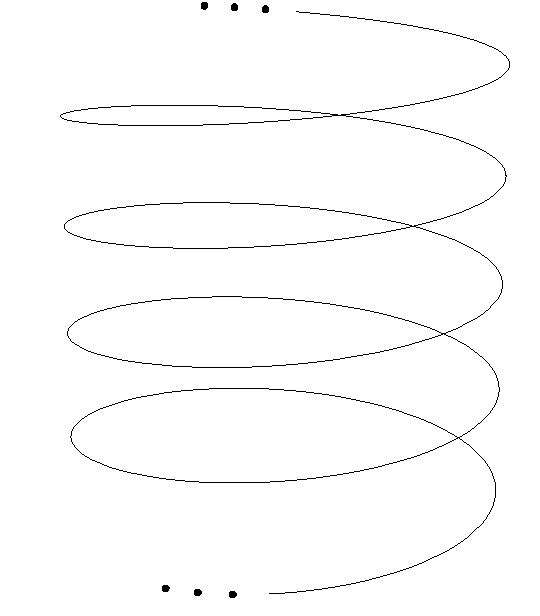
\includegraphics[width=3em]{covering_space.pdf}} \ar[d]^p \\
        I \ar[r] & 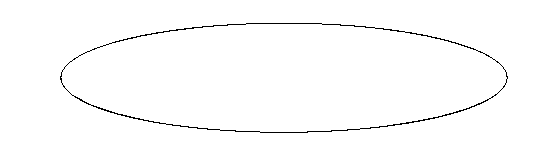
\includegraphics[width=3em]{circle.pdf}
      }
      \qquad\qquad\qquad
      \xymatrix{
        \{0\} \ar[r] \ar@{^(->}[d] & \mathbb R \ar[d]^p \\
        I \ar[r] & S^1
      }
    \]
  \end{example}
  
  
  \begin{example}
    The statement that we may lift any homotopy from the circle to its covering space is the statement that a lift of the following diagram (shown pictorally on the left and symbolically on the right) exists:
    \[
      \xymatrix{
        {\raisebox{0em}[1.5\height][\dimexpr1.5\height+\depth\relax]{$\bullet$}}
           \ar[r] \ar@{^(->}[d] & \raisebox{-0.5\height}{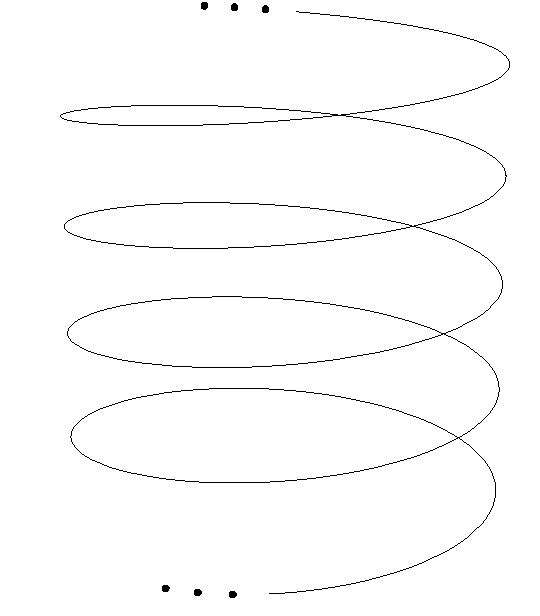
\includegraphics[width=3em]{covering_space.pdf}} \ar[d]^p \\
        {\raisebox{-0.3\height}{\resizebox{2em}{!}{\mbox{$\square$}}}} \ar[r] & 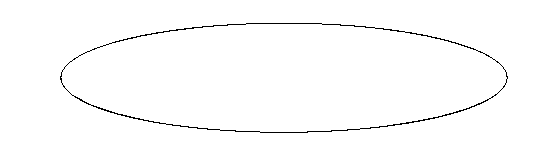
\includegraphics[width=3em]{circle.pdf}
      }
      \qquad\qquad\qquad
      \xymatrix{
        \{(0, 0)\} \ar[r] \ar@{^(->}[d] & \mathbb R \ar[d]^p \\
        I\times I \ar[r] & S^1
      }
    \]
  \end{example}
  
\section{Topological Background}
  %\begin{defn}[Weak Homotopy Equivalence]
  %  Let $X$ and $Y$ be topological spaces.  For any map $f : X \to Y$, for each basepoint $x\in X$, we may define the map $f_* : \pi_n(X, x) \to \pi_n(Y, f(x))$ by composition with $f$.  Then $f$ is a \defnlabel{weak homotopy equivalence} if $f_*$ is a bijection of pointed sets for $n = 0$ and an isomorphism of groups for $n \ge 1$.
  %  
  %  Informally, two spaces are weakly homotopy equivalent if they are isomorphic as sets, and there is no way to distinguish them by any higher-dimensional analog of loops.
  %\end{defn}
  
  Let $X$ and $Y$ be topological spaces.
  
  \begin{defn}[Homotopic Maps]
    Let $f$ and $g$ be continuous maps $X \to Y$.  We say that $f$ and $g$ are \defnlabel{homotopic} if there exists a family of maps $h_t : X \to Y$ such that $h_0 = f$, $h_1 = g$, and the map $h : I \times X \to Y$ given by $h(t, x) = f_t(x)$ is continuous in $t$ and $x$.
  \end{defn}
  
  \begin{defn}[Homotopy Equivalence]
    Let $f: X \to Y$ and $g: Y \to X$ be continuous maps.  If $gf$ is homotopic to $\id_X$ and $fg$ is homotopic to $\id_Y$, then we say that $X$ and $Y$ are \defnlabel{homotopy eqivalent}, and we call $f$ and $g$ \defnlabel{homotopy equivalences}.
  \end{defn}
  
  %\begin{defn}[Serre Fibration]
  %  A map $p : X \to Y$ is called a \defnlabel{Serre fibration} if, for each CW-complex $A$, the map $p$ has the \defnref{right lifting property} with respect to the inclusion $A \times 0 \to A \times [0, 1]$.  That is, $p$ is a Serre fibration if for any CW-complex $A$ and any maps $f$ and $g$, there is a map $h$ which makes the following diagram commute:
  %  \[
  %    \xymatrix{
  %      A \times 0 \ar[r]^f \ar@{^(->}[d]_-i & X \ar[d]^-p \\
  %      A \times I \ar[r]^-g \ar@{.>}[ur]^-h & Y
  %    }
  %  \]
  %\end{defn}
  
  \begin{defn}[Closed Hurewicz Cofibration]
    Let $B$ be a topological space and let $A$ be a subspace of $B$.  We call the subspace inclusion $i : A \hookrightarrow B$ a \defnlabel{closed Hurewicz cofibration} if $A$ is a closed subspace of $B$ and $i$ has the homotopy extension property.  The map $i$ has the \defnlabel{homotopy extension property} if a lift exists in the every commutative diagram of the following form for every topological space $Y$:
    \[
      \xymatrix{
        B \times 0 \cup A \times I \ar[r] \ar[d] & Y \ar[d] \\
        B \times I \ar[r] & {*}
      }
    \]
  \end{defn}
  
  FIX (DESCRIBE/INUITIVE/EXAMPLES)
  
  \begin{defn}[Hurewicz Fibration]
    A map $p : X \to Y$ is called a \defnlabel{Hurewicz fibration} if $p$ has the \defnlabel{homotopy lifiting property}, i.e. if, for each topological space $A$, the map $p$ has the \defnref{right lifting property} with respect to the inclusion $A \times 0 \to A \times [0, 1]$, i.e. if there is always a map $h$ which makes the following diagram commute:
    \[
      \xymatrix{
        A \times 0 \ar[r] \ar@{^(->}[d] & X \ar[d]^-p \\
        A \times I \ar[r] \ar@{.>}[ur]^-h & Y
      }
    \]
  \end{defn}
  
  FIX (DESCRIBE/INUITIVE/EXAMPLES)
  
  
\section{Model Categories}
  I first define a model category, using essentially the same terminology as \cite{dwyer1995homotopy}, before elaborating on each of the axioms in a little more detail.
  
  \begin{defn}[Model Category]
    Let \cat C be a category with three distinguished classes of morphisms:
    \begin{itemize}
      \item \defnlabel{weak equivalences} ($\stackrel{\sim}{\to}$)
      \item \defnlabel{fibrations} ($\twoheadrightarrow$)
      \item \defnlabel{cofibrations} ($\hookrightarrow$)
    \end{itemize}
    Suppose further that each class of morphisms is closed under composition and must contain all identity morphisms.  A map which is both a fibration (respectively cofibration) and a weak equivalence is called an \defnlabel{acyclic fibration} (respectively \defnlabel{acyclic cofibration}).
    We call $\cat C$ a \defnlabel{model category} if $\cat C$ satisfies the following axioms:
    \begin{enumerate}[\bf{MC}1]
      \item \defnref[small limits]{Finite limits and colimits exist} in \cat C.
      \item If $f$ and $g$ are morphisms in $\cat C$ such that $gf$ is defined, and two of $f$, $g$, and $gf$ are weak equivalences, then so is the third.
      \item If $f$ is a \defnref{retract} of $g$, and $g$ is a weak equivalence, fibration, or cofibration, then so is $f$.
      \item Cofibrations $i$ have the \defnref{left lifting property} with respect to all acyclic fibrations $p$.  Fibrations $p$ have the \defnref{right lifting property} with respect to all acyclic cofibrations $i$.
      \item All maps $f$ can be factored in two ways: (i) $f = pi$, where $i$ is a cofibration and $p$ is an acyclic fibration, and (ii) $f = pi$, where $i$ is an acyclic cofibration and $p$ is a fibration.
    \end{enumerate}
  \end{defn}
  
  \begin{example}[\texorpdfstring{\cat{Top}}{Top}]
    The category \cat{Top} of topological spaces can be given a model category structure where a map $f : X \to Y$ is
    \begin{itemize}
      \item a \emph{weak equivalence} if $f$ is a homotopy equivalence,
      \item a \emph{cofibration} if $f$ is a closed Hurewicz cofibration, and 
      \item a \emph{fibration} if $f$ is a Hurewicz fibration.
    \end{itemize}
  \end{example}
  
  \subsection*{MC1}
    Finite limits and colimits exist in \cat C.
    
    In a very rough sense, this axiom asserts that we are capable of taking two objects and constructing their product and coproduct; in \cat{Set} and \cat{Top}, all limits can be constructed by taking products and subspaces, and all colimits can be constructed by taking disjoint unions and and equivalence classes.
    
    FIX (TALK ABOUT WHY WE NEED THIS)
  \subsection*{MC2}
    If $f$ and $g$ are morphisms in $\cat C$ such that $gf$ is defined, and two of $f$, $g$, and $gf$ are weak equivalences, then so is the third.
    
    In a model category, weak equivalences are our notion of ``equality''.  This axiom asserts that weak equivalence is transitive (if $X$ is weakly equivalent to $Y$ and $Y$ is weakly equivalent to $Z$, then $X$ is weakly equivalent to $Z$).
    
    FIX (ADD WHY THE AXIOM IS THIS WAY, AND NOT WEAKER OR STRONGER)
  \subsection*{MC3} If $f$ is a \defnref{retract} of $g$, and $g$ is a weak equivalence, fibration, or cofibration, then so is $f$.
  
    FIX (ADD DIAGRAM, EXPLAIN IN MORE DETAIL)
    
  \subsection*{MC4} Cofibrations $i$ have the \defnref{left lifting property} with respect to all acyclic fibrations $p$.  Fibrations $p$ have the \defnref{right lifting property} with respect to all acyclic cofibrations $i$.
    
    FIX (ADD EXPOSITION)
    
  \subsection*{MC5} All maps $f$ can be factored in two ways: (i) $f = pi$, where $i$ is a cofibration and $p$ is an acyclic fibration, and (ii) $f = pi$, where $i$ is an acyclic cofibration and $p$ is a fibration.
  
    FIX (ADD EXPOSITION)

%\section{Homotopy}
%  \subsection{Cylinder Objects}
%  \subsection{Left Homotopy}
%  \subsection{Path Object}
%  \subsection{Right Homotopy}
%  \subsection{Homotopic Maps}
  
%\section{Further Reading}
%  FIX

\section{Solutions to the Exercises}
    \begin{soln*}[to \autoref{xca:initial_terminal_unique}] \label{sol:initial_terminal_unique}
      The initial and terminal objects of a category, if they exist, are unique up to unique \defnref{isomorphism}.
      
      If $*$ and $*'$ are two terminal objects of $\cat C$, then there is a unique morphism $f: *' \to *$ (because $*$ is terminal) and a unique morphism $g : * \to *'$ (because $*'$ is terminal).  Furthermore, we must have $gf = \id_{*'}$ and $fg = \id_{*}$ (because the idenity maps are the unique maps from $* \to *$ and $*' \to *'$).  Thus $*$ and $*'$ are \defnref{isomorphic}, and there is a unique \defnref{isomorphism} between them.
    \end{soln*}
    
    \begin{soln*}[to \autoref{xca:functor_commutative_diagram}] \label{sol:functor_commutative_diagram}
      Saying that the diagram
      \[
        \xymatrix{
          \Hom_{\cat C}(Y, Z) \ar[r] \ar[d] & \Hom_{\cat D}(F(Y), F(Z)) \ar[d] \\
          \Hom_{\cat C}(X, Z) \ar[r] & \Hom_{\cat D}(F(X), F(Z))
        }
      \]
      commutes is equivalent to saying that the two maps $\Hom_{\cat C}(Y, Z)\rightrightarrows \Hom_{\cat D}(F(X), F(Z))$ are equivalent.
      
      Specifying a morphism $f: X \to Y$ naturally specifies a unique map $\Hom_{\cat C}(Y, Z) \to \Hom_{\cat C}(X, Z)$; for any map $h : Y \to Z$, we get a map $hf : X \to Z$ by composing $h$ with $f$.  The top-right path is given by mapping $h\in \Hom_{\cat C}(Y, Z)$ to $F(h)$ and then composing it with $F(f)$, giving $F(h)F(f)$.  The bottom-right path is given by composing $h\in \Hom_{\cat C}(Y, Z)$ with $f$ to get $hf : X \to Z$, and then applying $F$ to get $F(hf)$.  Saying that these two paths are the same is equivalent to saying that $F(hf) = F(h)F(f)$, i.e., that the functor $F$ is compatible with composition of morphisms.
    \end{soln*}
    
    \begin{soln*}[to \autoref{xca:hom_op}] \label{sol:hom_op}
      Consider objects $X$, $Y$, $X'$, and $Y'$ in $\cat C$.  The functor $\Hom_{\cat C}(-, -)$ sends $(X, Y) \mapsto \Hom_{\cat C}(X, Y)$ and $(X', Y') \mapsto \Hom_{\cat C}(X', Y')$.  We want to know how $\Hom_{\cat C}(-, -)$ acts on morphisms.
      
      Suppose we have a morphism $(f^\text{op}, g)$ in $\cat C^\text{op} \times \cat C$, where $f^\text{op} : X \to X'$ and $g : Y \to Y'$.  We want an induced morphism from $\Hom_{\cat C}(X, Y)$ to $\Hom_{\cat C}(X', Y')$, given by specifying how each map $h: X \to Y$ becomes a map $h': X' \to Y'$.  The natrual way to define a map $X' \to Y'$ is by composing $h$ with a map $X' \to X$ on one side and $Y \to Y'$ on the other, so that we have the map
      \[
        h' : X' \xrightarrow{f} X \xrightarrow{h} Y \xrightarrow{g} Y'.
      \]
      Thus we see that we need a map $f : X' \to X$, which is the same as saying that we need a map $f^\text{op} : X \to X'$.  Hence we need a map from $\cat C^\text{op}$ in the first argument and a map from $\cat C$ in the second.
      
      Diagramatically, this is
      
    \[
      \xymatrix{
        X \ar[r]^h & Y \ar[d]^g \\
        X' \ar[u]_{f} \ar[r]^{h'} & Y' \\
      }
    \]
      
    \end{soln*}
    
    \begin{soln*}[to \autoref{xca:product_coproduct}] \label{sol:product_coproduct}
      The colimit of the diagram
      \[
        \{-4, 12, 183\}\qquad \{0, 12, 36\}
      \]
      is the set $C$ and map $t$ such that for each $X$ and each map $s$, there exists a unique $s'$ which makes the following diagram commute:
      \[
      \xymatrix{
        \{-4, 12, 183\}\ar@/_/[ddr]_s\ar[dr]^t && \{0, 12, 36\}\ar@/^/[ddl]^s\ar[dl]_t \\
        & C\ar@{.>}[d]^{s'}& \\
        &X&
      }
    \]
    If $s$ sends each element of each set to a distinct element of $X$, then $t$ must similarly send each element to a distinct element of $C$, so that $s't = s$.  Additionally, if we specify where every element of the two sets goes in $s = s't$, then we have fully (and uniquely) specified $s$.  Thus, the colimit is the set $C = \{-4, 12, 183\}\sqcup \{0, 12, 36\} = \{-4, 12, 183, 0, 12, 36\}$, and the map $t$ is given by inclusion.
    
    
      The limit of the diagram
      \[
        \{-4, 12, 183\}\qquad \{0, 12, 36\}
      \]
      is the set $L$ and map $t$ such that for each $X$ and each map $s$, there exists a unique $s'$ which makes the following diagram commute:
      \[
      \xymatrix{
        \{-4, 12, 183\} && \{0, 12, 36\} \\
        &L\ar[ul]_t\ar[ur]^t& \\
        &X\ar@/^/[uul]^s\ar@/_/[uur]_s\ar@{.>}[u]_{s'}&
      }
    \]
    If, for every pair of elements (one in the left set, one in the right set), $s$ sends some element of $X$ to the first of that pair on the left and the second of that pair on the right, then we must have a distinct object in $L$ for each such pair, so that $ts' = s$.  Additionally, if we specify where every pair of elements comes from in $X$, then we have fully (and uniquely) specified $s$.  Thus, the limit is the set $L = \{-4, 12, 183\}\times \{0, 12, 36\}$, and the map $t$ is given by projection (i.e., $(a, b) \mapsto a$ and $(a, b) \mapsto b$).
    \end{soln*}
  
\nocite{*}
\bibliographystyle{plain}
\bibliography{quillen_model_structures}
\end{document}